%%%%%%%%%%%%%%%%%% ANOTHER LECTURE

\chapter{Kaluza--Klein Reduction}

The Kaluza--Klein program aims to obtain the $d$-dimensional theory obtained by reducing a $D$-dimensional one. The original idea was to obtain four-dimensional gravity and electrodynamics, from five-dimensional gravity... All of it in the context of general relativity.

In the following the dimensional reduction of the action of a scalar field on $D+1$-dimension to $D$-dimensions is shown, and later, the reduction of $D+1$-dimensional gravity on a $S^1$.  A nice reference to the program is~\cite{PopeKK}.

\section{Reduction of a Scalar Field}

On this section the reduction of a massless, real, scalar field is performed on different manifolds. All over the section it is assumed that the total manifold is nothing but a Cartesian product of two other manifolds.



\subsection{Scalar Field Reduced on $S^1$}
\label{sec:KKs:s1}

Consider the equation of motion of a massless (real) scalar field $\Phi$ on $D+1$-dimensions, 
\begin{equation}
  \Box^{(D+1)} \Phi = 0.
\end{equation}
Assume that $M^{D+1} = M^D \times S^1$. Then,  the differential operator can be separated  into a $D$-dimensional part plus the extra dimension,
\begin{equation}
  \( \Box^{(D)} + \pa{\xi}^2 \) \Phi = 0.
  \label{KK-s-eq:s1}
\end{equation}

Now, one propose the Kaluza--Klein ansatz, i.e., the scalar field can be expanded as a series on the basis of eigenfunctions on $S^1$,
\begin{equation}
  \Phi(x,\xi) = \sum_n \phi_n(x) e^{\imath \frac{n}{R} \xi},
  \label{KK-scalar:s1}
\end{equation}
where $R$ is the radius of the extra dimension.

Substituting the expansion in Eq.~\eqref{KK-scalar:s1} into~\eqref{KK-s-eq:s1}, yields
\begin{equation}
  \[ \Box^{(D)} - \( \frac{n}{R} \)^2 \] \phi_n(x) = 0 \qquad \forall \; n \in \Z.
  \label{KK-eq-s1}
\end{equation}

Comparing with the generic Klein-Gordon equation,
\begin{equation}
  \[ \Box^{(D)} - m_{\text{eff}}^2 \] \phi_n = 0, \qquad \text{with} \qquad m_{\text{eff}} = \frac{ \abs{n} }{ R },
  \label{KKs-m:s1}
\end{equation}
one concludes that Eq.~\eqref{KK-eq-s1}  represents  a tower of infinite massive scalar fields in $D$ dimensions; doubly degenerated because of the blindness on the sign of $n$, plus a single massless scalar field, corresponding to $n = 0$.

\begin{center}
  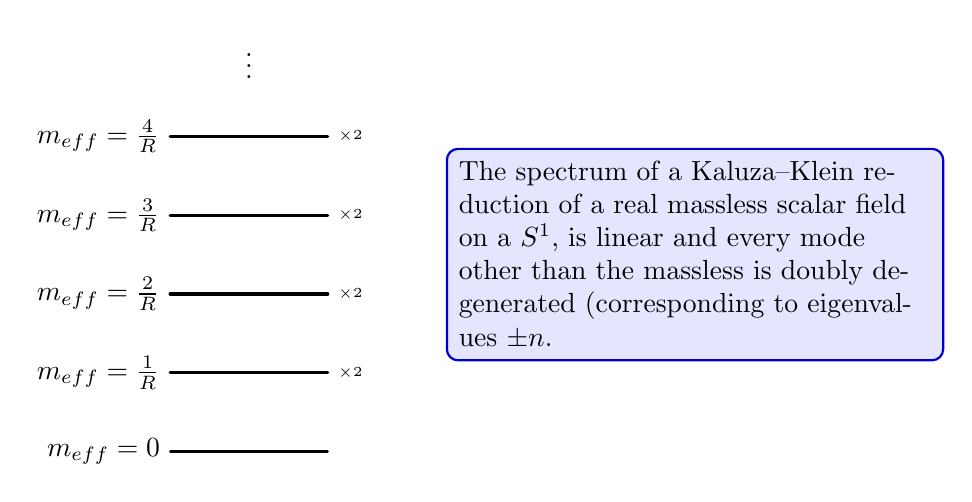
\begin{tikzpicture}[thick,line cap=round,
      % Styles
      axes/.style=,
      important line/.style={very thick},
      information text/.style={rounded corners,draw=blue!80!black,fill=blue!10,inner sep=1ex}]
    
    \draw (0,0) node[anchor=east] {$m_{\text{eff}} = 0$} -- (2,0);
    \foreach \y in {1,2,...,4}
    \draw[important line] (0,\y) node[anchor=east] {$m_{\text{eff}} = \frac{\y}{R}$} -- (2,\y);
    \foreach \y in {1,2,...,4}
    \node[anchor=west] at (2,\y) {{\tiny $ \times 2$}};

    \node at (1,5) {$\vdots$};

    \draw[xshift=3.5cm,yshift=2.5cm]
    node[right,text width=6cm,information text]
    {The spectrum of a Kaluza--Klein reduction of a real massless scalar field on a $S^1$, is linear and every mode other than the massless is doubly degenerated (corresponding to eigenvalues $\pm n$.};
  \end{tikzpicture}
\end{center}

\subsection{Scalar Field Reduced on $S^2$}
\label{sec:KKs:s2}

One can follow the previous procedure to compute the \KK of a massless real scalar field on $S^2$. Thus, assuming that $M^{D+2} = M^D \times S^2$, the differential operator separates on,
\begin{equation}
  \( \Box^{(D)} + \Lap \) \Phi = 0.
  \label{KKs-eq:s2}
\end{equation}
Then, the \KK ansatz is done as an expansion on eigenfunctions of the 2-dimensional Laplacian on spherical coordinates, i.e., spherical harmonics, as
\begin{equation}
  \Phi(x,\xi) = \sum_{l,m} \phi_{l,m}(x) \, Y^{lm}(\xi),
\end{equation}
where $Y^{lm}$ satisfy
\begin{equation}
  \Lap Y^{lm} = - \frac{ l(l+1) }{ R^2 } Y^{lm}.
\end{equation}

Therefore, Eq.~\eqref{KKs-eq:s2} yields
\begin{equation}
  \[ \Box^{(D)} - \frac{ l(l+1) }{ R^2 } \] \phi_{l,m}(x) = 0.
  \label{KK-eq-s2}
\end{equation}
Equation~\eqref{KK-eq-s2} represents a \KK tower composed by: a single massless scalar field, corresponding to $l = 0$; and $(2l + 1)$-degenerated massive scalar fields with and effective mass
\begin{equation}
  m_{\text{eff}} = \frac{ \sqrt{ l(l+1) } }{ R }.
  \label{KKs-m:s2}
\end{equation}

\begin{center}
  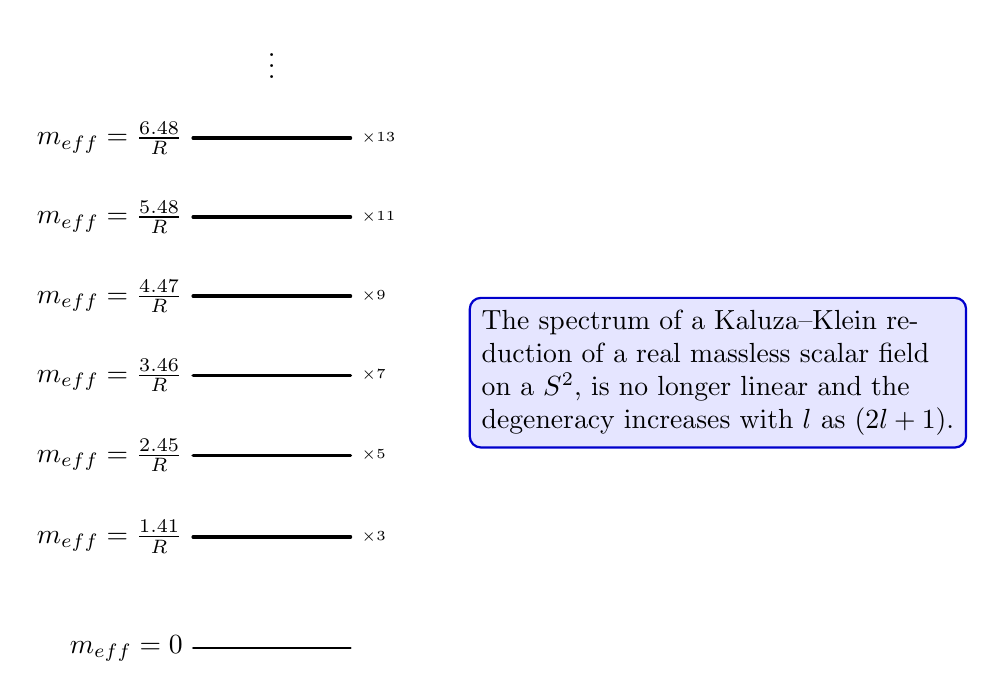
\begin{tikzpicture}[thick,line cap=round,
      % Styles
      axes/.style=,
      important line/.style={very thick},
      information text/.style={rounded corners,draw=blue!80!black,fill=blue!10,inner sep=1ex}]
    \pgfkeys{/pgf/number format/.cd,fixed,precision=2}

    \draw (0,0) node[anchor=east] {$m_{\text{eff}} =0$} -- (2,0);
    \foreach \y/\m in {1/3,2/5,3/7,4/9,5/11,6/13}
             {
               \draw[important line] (0,{sqrt(\y*\y + \y) }) node[anchor=east] {$m_{\text{eff}} =\frac{\pgfmathparse{sqrt(\y*\y + \y) }\pgfmathprintnumber{\pgfmathresult}}{R}$} -- (2,{sqrt(\y*\y + \y) }) node[anchor=west]  {{\tiny $ \times\m$}};
             }
             \node at (1,7.5) {$\vdots$};

             \draw[xshift=3.5cm,yshift=3.5cm]
             node[right,text width=6cm,information text]
             {The spectrum of a Kaluza--Klein reduction of a real massless scalar field on a $S^2$, is no longer linear and the degeneracy increases with $l$ as $(2l+1)$.};
  \end{tikzpicture}
\end{center}

\subsection{Scalar Field Reduced on $T^2$}
\label{sec:KKs:t2}

Once more, inspired in the previous procedure, and using the fact that $T^2 = S^1 \times S^1$, the differential operator separates on,
\begin{equation}
  \( \Box^{(D)} + \pa{\xi_1}^2 + \pa{\xi_2}^2 \) \Phi = 0,
  \label{KKs-eq:t2}
\end{equation}
and the \KK ansatz is
\begin{equation}
  \Phi(x, \xi) = \sum_{m,n} \phi_{m,n}(x) \, e^{\imath \( \frac{m}{R_1} \xi_1 + \frac{n}{R_2} \xi_2 \)},
  \label{KK-scalar:t2}
\end{equation}
where $R_1$ and $R_2$ are the radii of the torus.

Substituting the expansion in Eq.~\eqref{KK-scalar:t2} into~\eqref{KKs-eq:t2}, yields
\begin{equation}
  \[ \Box^{(D)} - \( \frac{m}{R_1} \)^2 - \( \frac{n}{R_2} \)^2 \] \phi_{m,n}(x)= 0 \qquad \forall \; m, n \in \Z.
  \label{KK-eq-t2}
\end{equation}

Equation~\eqref{KK-eq-t2} represents a tower of \KK modes which contains a massless singlet, and infinite massive modes whose degeneracy depend on the relation between the integers $m,n$ and the radii $R_1$ and $R_2$. The effective mass for the \KK modes is
\begin{equation}
  m_{\text{eff}} =  \sqrt{ \( \frac{m}{R_1} \)^2 + \( \frac{n}{R_2} \)^2 }.
  \label{KKs-m:t2}
\end{equation}

\begin{center}
  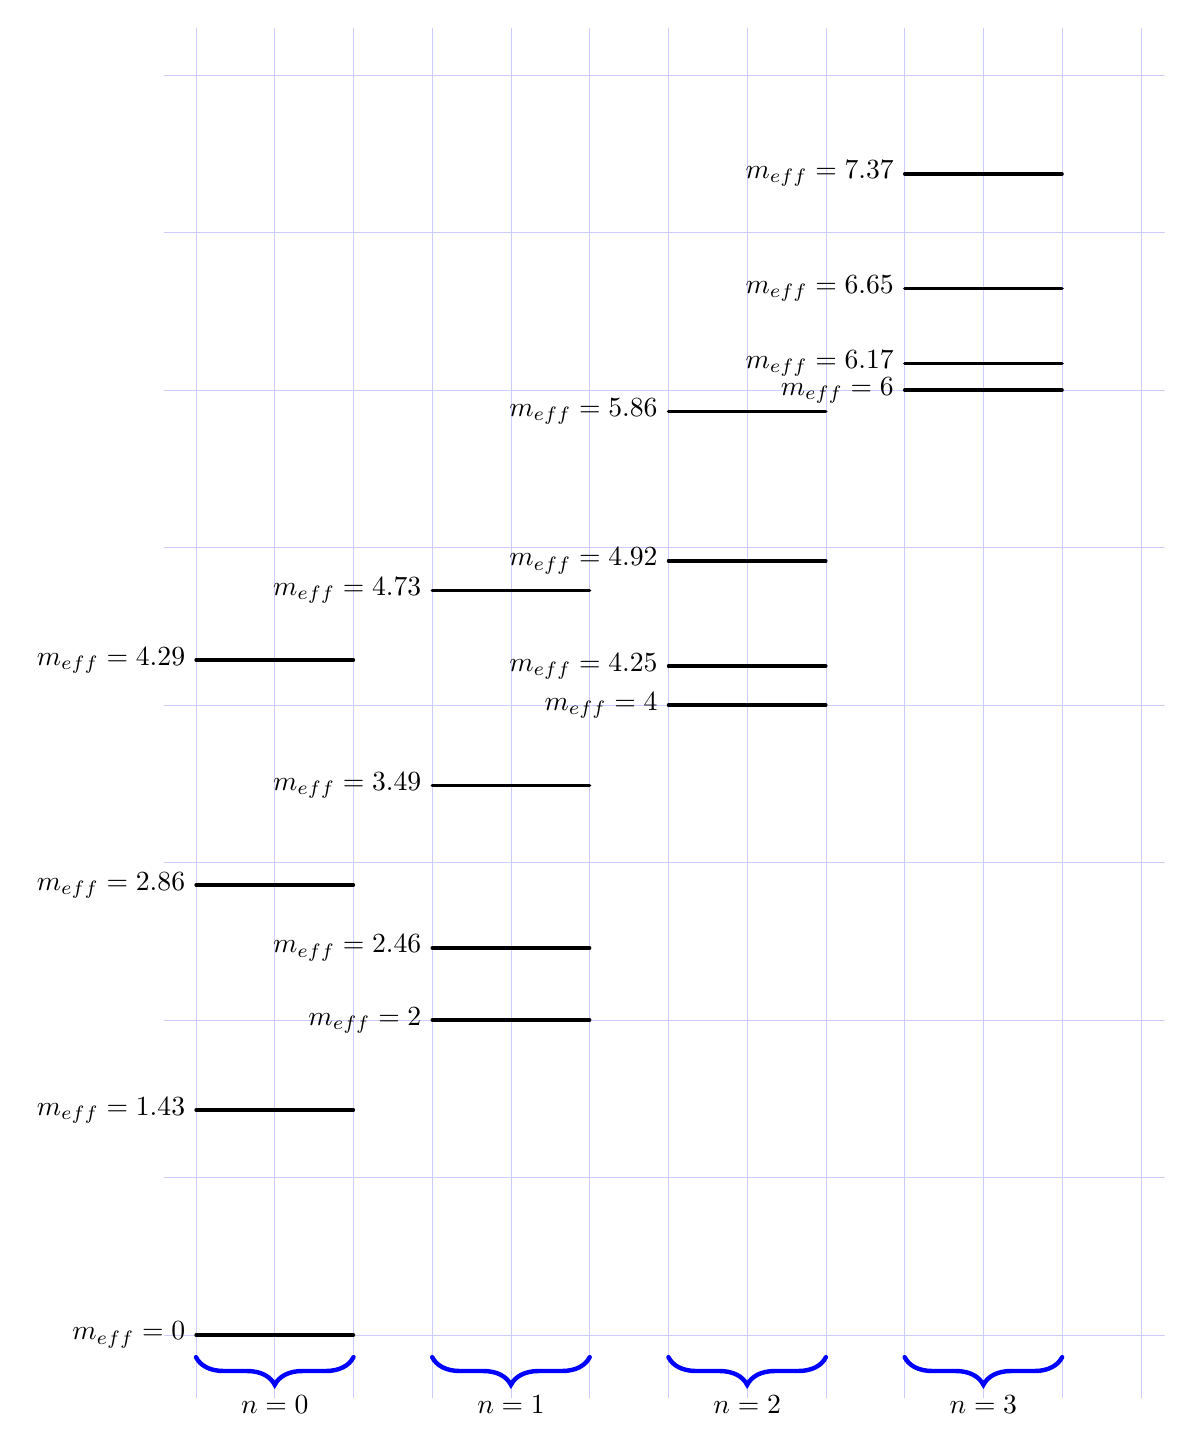
\begin{tikzpicture}[thick,line cap=round,yscale=2,
      % Styles
      axes/.style=,
      important line/.style={very thick},
      information text/.style={rounded corners,draw=blue!80!black,fill=blue!10,inner sep=1ex}]
    \pgfkeys{/pgf/number format/.cd,fixed,precision=2}

    \pgfmathsetmacro{\r}{.7}
    \pgfmathsetmacro{\R}{.5}
    
    \draw[help lines, color=blue!20,step=1cm] (-.4,-.4) grid (12.3,8.3);

    %\draw (0,0) node[anchor=east] {$m_{\text{eff}} =0$} -- (2,0);
    \foreach \n in {0,1,2,3}  {
      \foreach \m in {0,1,...,3} {
        \draw[important line,xshift=3*\n cm] (0,{sqrt((\m/\r)^2 + (\n/\R)^2)}) node[anchor=east] {$m_{\text{eff}} = \pgfmathparse{sqrt((\m/\r)^2 + (\n/\R)^2) }\pgfmathprintnumber{\pgfmathresult}$} -- (2,{sqrt((\m/\r)^2 + (\n/\R)^2)});
      }
      \draw [decorate,decoration={brace,amplitude=10pt,mirror},ultra thick,color=blue,yshift=-4pt,xshift=3*\n cm] (0,0) -- (2,0) node [black,midway,yshift=-0.6cm] { $n = \n$};
    }    
  \end{tikzpicture}
\end{center}


\section{Kaluza--Klein Reduction on $S^1$}

\begin{equation}
  \de{\hat{s}}^2 = e^{2\alpha\phi} \de{s}^2 + e^{2 \beta \phi} \left( \de{\xi} + \Ag[1] \right)^2,
\end{equation}

\begin{equation}
  \VIF{a} = 
  \begin{cases}
    \hvif{a} = e^{\alpha\phi} \vif{a}\\
    \hvif{D} = e^{\beta\phi} \left( \df[\xi] + \Ag*[1] \right)
  \end{cases},
\end{equation}

From the first Maurer-Cartan equation,
\begin{equation}
  \df \VIF{a} + \SPIF{a}{b} \we \VIF{b} = \TF{a} = 0,
\end{equation}
the spin connection can be calculated.
\begin{align}
  \df\hvif{D}
  &= e^{\beta \phi} \left[ \beta \; \df[\phi] \we \left( \df[\xi] + \Ag*[1] \right) + \df\Ag*[1] \right] \nonumber\\
  &= e^{\beta \phi} \left[ -\beta \left( \df[\xi] + \Ag*[1] \right) \we \df[\phi] + \df \Ag*[1] \right] \nonumber\\
  &= e^{\beta \phi} \left[ -\beta \pa{a}\phi \left( \df[\xi] + \Ag*[1] \right) \we \vif{a} + \Fg*[2] \right] \nonumber\\
  &= - \beta e^{-\alpha \phi} \pa{a} \phi \; \hvif{D} \we \hvif{a} - \frac{1}{2} e^{(\beta - 2\alpha) \phi} \Fg_{a b} \; \hvif{b} \we \hvif{a},
\end{align}
from where one gets,
\begin{equation}
  \hspif{D}{a} = \beta e^{-\alpha \phi} \pa{a} \phi \, \hvif{D} + \frac{1}{2} e^{(\beta - 2\alpha) \phi} \Fg_{a b} \, \hvif{b}.
\end{equation}

On the other hand,
\begin{equation}
  \hspif{a}{b} \we \hvif{b} = - \df\hvif{a} - \hspif{a}{D} \we \hvif{D}.
\end{equation}
Since,
\begin{align}
  \df\hvif{a} 
  &= e^{\alpha \phi} \left[ \alpha \, \df[\phi] \we \vif{a} +  \df\vif{a} \right] \nonumber\\
  &= e^{\alpha \phi} \left[ -\alpha \, \vif{a} \we \df[\phi] -  \spif{a}{b} \we \vif{b} \right] \nonumber\\
  &= -\alpha e^{-\alpha \phi} \pa{b} \phi \; \hvif{a} \we \hvif{b} - \spif{a}{b} \we \hvif{b},
\end{align}
then,
\begin{align}
  \hspif{ab}{}
  &= \spif{ab}{} + \alpha e^{- \alpha \phi} \pau{b} \phi \, \hvif{a} - \frac{1}{2} e^{(\beta - 2\alpha) \phi} \Fg^{a b} \, \hvif{D} \nonumber\\
  &= \spif{ab}{} + \alpha e^{-\alpha \phi} \left( \pau{b} \phi \, \hvif{a} - \partial^{a} \phi \, \hvif{b} \right) - \frac{1}{2} e^{(\beta - 2\alpha) \phi} \Fg^{a b} \, \hvif{D}.
\end{align}

Now, the second Maurer-Cartan equation,
\begin{equation}
  \df\SPIF{a}{b} + \SPIF{a}{c} \we \SPIF{c}{b} = \RIF{a}{b}.
\end{equation}

\begin{align}
  \df\hspif{D a}{} 
  &= \beta \, \df \left( e^{-\alpha \phi} \pau{a} \phi \,\hvif{D} \right) + \frac{1}{2} \df \left( e^{(\beta - 2\alpha) \phi} \Fg^a{}_{b} \, \hvif{b} \right) \nonumber\\
  &= \beta e^{-\alpha\phi} \, \left[ -\alpha \pau{a} \phi \, \df[\phi] \we \hvif{D} + \pau{a} \, \df[\phi] \we \hvif{D} + \pau{a} \phi \, \df \hvif{D} \right] \notag \\
  &\quad + \frac{1}{2} e^{(\beta - 2\alpha) \phi} \left[ (\beta-2\alpha) \Fg^a{}_{b} \, \df[\phi] \we \hvif{b} + \df[\Fg^a{}_{b}] \we \hvif{b} + \Fg^a{}_{b} \, \df[\hvif{b}] \right] \nonumber \\
  &= \beta e^{-\alpha\phi} \left[ -\alpha \pau{a} \phi \pa{b} \phi \, \vif{b} \we \hvif{D} + \pau{a} \pa{b} \phi \, \vif{b} \we \hvif{D} + \pau{a} \phi \, \hspif{D}{b} \we \hvif{b} \right] \notag \\
  &\quad + \frac{1}{2} e^{(\beta - 2\alpha) \phi} \left[ (\beta - 2\alpha) \Fg^a{}_b \pa{c} \phi \, \vif{c} \we \hvif{b} + \pa{c} \Fg^a{}_b \, \vif{c} \we \hvif{b} + \Fg^a{}_b \, \hspif{b}{\hat{c}} \we \VIF{c} \right] \nonumber \\
  &= \beta (\beta - \alpha) e^{-2\alpha \phi} \pau{a} \phi \pa{b} \phi \, \hvif{b} \we \hvif{D} + \beta e^{-2\alpha \phi} \pau{a} \pa{b} \phi \, \hvif{b} \we \hvif{D}  \notag \\
  &\quad - \frac{\beta-\alpha}{2} e^{(\beta - 3\alpha) \phi} \Fg^a{}_b \pa{c} \phi\, \hvif{b} \we \hvif{c} + \frac{\beta}{2} e^{(\beta - 3\alpha) \phi} \pau{a} \phi \Fg_{bc} \, \hvif{b} \we \hvif{c} \nonumber \\
  &\quad -\frac{1}{2} e^{(\beta - 3\alpha) \phi} \pa{c} \Fg^a{}_b \, \hvif{b} \we \hvif{c} - \frac{1}{2} e^{(\beta - 2\alpha) \phi} \Fg^a{}_b \, \spif{b}{c} \we \hvif{c},
\end{align}
and,
\begin{align}
  \hspif{D}{m} \we \hspif{m a}{}
  &= \left( \beta e^{-\alpha\phi} \pa{m} \phi \, \hvif{D} + \frac{1}{2} e^{(\beta - 2\alpha) \phi} \Fg_{m b} \, \hvif{b}  \right) \we \notag \\
  &\quad \left( \spif{m a}{} + \alpha e^{-\alpha\phi} \left( \pau{a} \phi \, \hvif{m} - \partial^{m} \phi \, \hvif{a} \right) - \frac{1}{2} e^{ (\beta - 2\alpha) \phi} \Fg^{m a} \, \hvif{D}  \right) \nonumber \\
  &= \beta e^{-\alpha\phi} \pa{m} \phi \, \hvif{D} \we \spif{m a}{} + \alpha \beta e^{-2\alpha\phi} \pa{m} \phi \, \hvif{D} \we \left( \pau{a} \phi \, \hvif{m} - \partial^{m} \phi \, \hvif{a} \right) \nonumber \\
  &\quad + \frac{1}{2} e^{ (\beta - 2\alpha) \phi } \Fg_{m b} \, \hvif{b} \we \spif{m a}{} + \frac{\alpha}{2} e^{ (\beta - 3\alpha) \phi } \Fg_{m b} \, \hvif{b} \we \left( \pau{a} \phi \, \hvif{m} - \partial^{m} \phi \, \hvif{a} \right) \nonumber\\
  &\quad -\frac{1}{4} e^{ 2 (\beta - 2\alpha) \phi } \Fg_{m n} \Fg^{m a} \, \hvif{n} \we \hvif{D}.
\end{align}
Therefore,
\begin{align}
  \hRif{D a}{}
  &= - \frac{1}{2} e^{(\beta-2\alpha)\phi} \( \Fg_{bc} \, \spif{ba}{} + \Fg^a{}_{b} \, \spif{b}{c} \) \we \hvif{c} - \beta e^{-\alpha\phi} \pa{m} \phi \, \spif{m a}{} \we \hvif{D} \notag \\
  &\quad + \[ \beta e^{-2\alpha\phi} \Big( (\beta - 2\alpha) \pa{b} \phi \pau{a} \phi + \pa{b} \pau{a} \phi \Big) - \frac{1}{4} e^{ 2 (\beta - 2\alpha) \phi} \Fg_{cb} \Fg^{ca} \] \, \hvif{b} \we \hvif{D} \notag \\
  &\quad + \frac{ e^{(\beta - 3\alpha) \phi} }{ 2 } \bigg[ (\beta - \alpha) \big( \pau{a} \phi \Fg_{mb} + \pa{m} \phi \Fg^a{}_b \big) + \pa{m} \Fg^a{}_b \bigg] \, \hvif{m} \we \hvif{b} \notag \\
  &\quad + \alpha \beta e^{-2\alpha\phi} \pa{m} \phi \partial^{m} \phi \, \hvif{a} \we \hvif{D} - \frac{\alpha}{2} e^{(\beta - 3\alpha) \phi} \pau{b} \phi \Fg_{bc} \, \hvif{c} \we \hvif{a}
\end{align}

The second term,
\begin{align}
  \df\hspif{ab}{}
  &= \df \spif{ab}{} + \df \[ \alpha e^{-\alpha\phi} \( \pau{b} \phi \, \hvif{a} - \pau{a} \phi \, \hvif{b} \) \] - \frac{1}{2} \df \[ e^{(\beta - 2\alpha) \phi} \Fg^{ab} \, \hvif{D} \]
  \notag \\
  &= \df \spif{ab}{} + \alpha^2 e^{-2\alpha\phi} \pa{c} \phi \( \pau{b} \phi \, \hvif{a} - \pau{a} \phi \, \hvif{b}\) \we \hvif{c}
  \notag \\
  &\quad - \alpha e^{-2\alpha\phi} \( \pa{c} \pau{b} \phi \, \hvif{a} - \pa{c} \pau{a} \phi \, \hvif{b}\) \we \hvif{c}  + \alpha e^{-\alpha\phi} \( \pau{b} \phi\, \df \hvif{a} - \pau{a} \phi \, \df \hvif{b} \)
  \notag \\
  &\quad - \frac{1}{2} e^{(\beta - 3\alpha) \phi} \[ (\beta - 2\alpha) \pa{c} \phi \Fg^{ab} + \pa{c} \Fg^{ab} \] \, \hvif{c} \we \hvif{D}
  \notag \\
  &\quad  - \frac{1}{2} e^{ (\beta - 2\alpha) \phi } \Fg^{ab} \, \df\hvif{D}
  \notag \\
  &= \df \spif{ab}{} - \alpha e^{-2\alpha\phi} \( \pa{c} \pau{b} \phi \, \hvif{a} - \pa{c} \pau{a} \phi \, \hvif{b} \) \we \hvif{c}
  \notag \\
  &\quad - \alpha e^{-\alpha\phi} \( \pau{b} \phi \, \spif{a}{m} - \pau{a} \phi \, \spif{b}{m} \) \we \hvif{m} - \frac{1}{4} e^{ 2(\beta - 2\alpha) \phi } \Fg^{ab} \Fg_{mn} \, \hvif{m} \we \hvif{n} \\
  &\quad - \frac{1}{2} e^{ (\beta - 3\alpha) \phi } \[ 2(\beta - \alpha) \pa{c} \phi \Fg^{ab} + \pa{c} \Fg^{ab} \] \, \hvif{c} \we \hvif{D},
  \notag
\end{align}
and 
\begin{align}
  \hspif{a}{D} \we \hspif{D b}{}
  &= - \(  \beta e^{-\alpha\phi} \pau{a} \phi \, \hvif{D} + \frac{1}{2} e^{(\beta-2\alpha)\phi} \Fg^{a}{}_m \, \hvif{m} \) \we \( \beta e^{-\alpha\phi} \pau{b} \phi \, \hvif{D} + \frac{1}{2} e^{(\beta - 2\alpha) \phi} \Fg^{b}{}_n \, \hvif{n} \)
  \notag\\
  &= + \frac{\beta}{2} e^{ (\beta - 3\alpha) \phi } \( \pau{a} \phi \Fg^{b}{}_m - \pau{b} \phi \Fg^{a}{}_m \) \, \hvif{m} \we \hvif{D}   -  \frac{1}{4} e^{ 2(\beta - 2\alpha) \phi } \Fg^{a}{}_m \Fg^{b}{}_n \, \hvif{m} \we \hvif{n}
\end{align}
\begin{align}
  \hspif{a}{c} \we \hspif{c b}{}
  &= \spif{a}{c} \we \spif{c b}{} + \frac{1}{2} e^{(\beta-2\alpha)\phi} \( \Fg^{a}{}_c \, \spif{cb}{} - \Fg^{b}{}_c \, \spif{ca}{}\) \we \hvif{D}
  \notag \\
  &\quad + \alpha e^{-\alpha\phi} \( \pau{b} \phi \, \spif{a}{c} \we \hvif{c} - \pau{c} \phi \, \spif{a}{c} \we \hvif{b} + \pau{c} \phi \, \spif{b}{c} \we \hvif{a} - \pau{a} \phi \, \spif{b}{c} \we \hvif{c}  \)
  \notag \\
  &\quad + \alpha^2 e^{-2\alpha\phi} \( \pau{b} \phi \pa{c} \phi \, \hvif{a} \we \hvif{c} - \pau{a} \phi \pa{c} \phi \, \hvif{b} \we \hvif{c} - \pau{c} \phi \pa{c} \phi \, \hvif{a} \we \hvif{b}  \)
  \notag \\
  &\quad + \frac{\alpha}{2} e^{(\beta - 3\alpha) \phi} \[ \Fg^b{}_c \( \pau{c} \phi \, \hvif{a} - \pau{a} \phi \, \hvif{c} \)  + \Fg^a{}_c \( \pau{b} \phi \, \hvif{c} - \pau{c} \phi \, \hvif{b}\) \] \we \hvif{D}.
\end{align}

Next, one can write the Lagrangian of the higher dimensional spacetime,
\begin{align}
  \Lag_{(D+1)}
  &= \frac{ \epsilon_{\hat{a}_1\hat{a}_2\cdots\hat{a}_{D+1}} }{ (D-1)! } \hRif{\hat{a}_1\hat{a}_2}{} \we \hvif{\hat{a}_3} \we \cdots \we \hvif{\hat{a}_{D+1}} \\[2ex]
  &= \underbrace{ 2 \frac{ \epsilon_{D a_1 a_2\cdots a_{D}} }{ (D-1)! } \hRif{D{a}_1}{} \we \hvif{{a}_2} \we \cdots \we \hvif{{a}_{D}} }_{\text{Term }I} \notag \\[2ex]
  & \quad + \underbrace{ \frac{ \epsilon_{a_1 a_2\cdots a_{D}D} }{ (D-2)! } \hRif{{a}_1{a}_2}{} \we \hvif{{a}_3} \we \cdots \we \hvif{{a}_{D}} \we \hvif{D} }_{\text{Term }II}.
\end{align}
Concentrate on the first term,
\begin{align}
  I
  &= 2(-1)^D \frac{ \epsilon_{a_1 a_2\cdots a_{D}} }{ (D-1)! }
  \notag \\
  &\qquad \bigg\{ \[ \beta e^{-2\alpha\phi} \big( (\beta - 2\alpha) \pa{b} \phi\pau{a_1} \phi + \pa{b} \pau{a_1} \phi \big) - \frac{1}{4} e^{2(\beta - 2\alpha) \phi} \Fg_{cb} \Fg^{ca_1} \] \, \hvif{b}
  \notag \\
  &\qquad + \beta e^{-\alpha\phi} \pa{m} \phi \, \spif{m a_1}{} + \alpha \beta e^{-2\alpha\phi} \pa{m} \phi \partial^{m} \phi \, \hvif{a} \bigg\} \we \hvif{D} \we \hvif{{a}_2} \we \cdots \we \hvif{{a}_{D}}
  \notag \\
  &= - 2 \frac{ \epsilon_{a_1 a_2\cdots a_{D}} }{ (D-1)! }
  \notag \\
  &\qquad \bigg\{ \[ \beta e^{-2\alpha\phi} \big( (\beta - 2\alpha) \pa{b} \phi \pau{a_1} \phi + \pa{b} \pau{a_1} \phi \big) - \frac{1}{4} e^{ 2(\beta - 2\alpha) \phi } \Fg_{cb} \Fg^{ca_1} \] \, \hvif{b}
  \notag \\
  &\qquad + \beta e^{-\alpha\phi} \pa{m}\phi \, \spif{m a_1}{} + \alpha \beta e^{-2\alpha\phi} \pa{m} \phi \partial^{m} \phi \, \hvif{a} \bigg\} \we \hvif{{a}_2} \we \cdots \we \hvif{{a}_{D}} \we \hvif{D}
  \notag \\
  &= -2 \frac{ \epsilon_{a_1 a_2\cdots a_{D}} }{ (D-1)! } e^{ \( (D-2) \alpha + \beta \) \phi }
  \notag \\
  &\qquad \bigg\{ \[ \beta \big( (\beta - 2\alpha) \pa{b} \phi \pau{a_1} \phi + \pa{b} \pau{a_1} \phi \big) - \frac{1}{4} e^{ 2(\beta - \alpha) \phi } \Fg_{cb} \Fg^{ca_1} \]\, \vif{b}
  \notag \\
  &\qquad + \beta \pa{m} \phi \, \(\spi{b}\)^{m a_1} \, \vif{b} + \alpha \beta \pa{m} \phi \partial^{m} \phi \, \vif{a_1} \bigg\} \we \vif{{a}_2} \we \cdots \we \vif{{a}_{D}} \we \df[\xi]
  \notag \\
  &= - 2 e^{\( (D-2) \alpha + \beta \) \phi} \bigg\{ \beta \big( (\beta - 2\alpha) \pa{b} \phi \pau{b} \phi + \pa{b} \pau{b} \phi \big)  - \frac{1}{4} e^{ 2(\beta  -\alpha) \phi } \Fg_{cb} \Fg^{cb}
  \notag \\
  &\qquad \quad + \beta \pa{m} \phi \, \(\spi{b}\)^{m b} + D \alpha \beta \, \pa{m}\phi \partial^{m}\phi \bigg\} \de{V_D}\de{\xi}
\end{align}

\begin{align}
  II
  &= \frac{ \epsilon_{a_1 a_2\cdots a_{D}D} }{ (D-2)! }
  \notag \\
  &\qquad \bigg\{ \Rif{a_1a_2}{} - \alpha e^{-2\alpha\phi} \( \pa{c} \pau{a_2} \phi \, \hvif{a_1} - \pa{c} \pau{a_1} \phi\, \hvif{a_2}\) \we \hvif{c}
  \notag \\
  &\qquad - \frac{1}{4} e^{ 2(\beta - 2\alpha) \phi} \( \Fg^{a_1a_2} \Fg_{mn} + \Fg^{a_1}{}_m \Fg^{a_2}{}_n \) \, \hvif{m} \we \hvif{n}
  \notag \\
  &\qquad + \alpha e^{-\alpha\phi} \( \pau{a_2} \phi \, \spif{a_1}{c} \we \hvif{c} - \pau{c} \phi \, \spif{a_1}{c} \we \hvif{a_2} + \pau{c} \phi \, \spif{a_2}{c} \we \hvif{a_1} - \pau{a_1} \phi \, \spif{a_2}{c} \we \hvif{c}  \)
  \notag \\
  &\qquad + \alpha^2 e^{-2\alpha\phi} \( \pau{a_2} \phi \pa{c} \phi \, \hvif{a_1} \we \hvif{c} - \pau{a_1} \phi \pa{c} \phi \, \hvif{a_2} \we \hvif{c} - \pau{c} \phi \pa{c} \phi \, \hvif{a_1} \we \hvif{a_2}  \)
  \notag \\
  &\qquad - \alpha e^{-\alpha\phi} \( \pau{a_2} \phi \, \spif{a_1}{m} - \pau{a_1} \phi \, \spif{a_2}{m}\) \we \hvif{m} \bigg\} \we \hvif{{a}_3} \we \cdots \we \hvif{{a}_{D}} \we \hvif{D}
  \notag \\
  &= \frac{ \epsilon_{a_1 a_2\cdots a_{D}} }{ (D-2)! } e^{ \( (D-2)\alpha + \beta \) \phi }
  \notag \\
  &\qquad \bigg\{ \Rif{a_1a_2}{} - \alpha \( \pa{c} \pau{a_2} \phi \, \vif{a_1} - \pa{c} \pau{a_1} \phi \, \vif{a_2}\) \we \vif{c}
  \notag \\
  &\qquad - \frac{1}{4} e^{ 2(\beta - \alpha) \phi } \( \Fg^{a_1a_2} \Fg_{mn} + \Fg^{a_1}{}_m \Fg^{a_2}{}_n \) \, \vif{m} \we \vif{n}
  \notag \\
  &\qquad + \alpha \( \pau{a_2} \phi \, \spif{a_1}{n} \we \vif{n} - \pau{c} \phi \, \spif{a_1}{c} \we \vif{a_2} + \pau{c} \phi \, \spif{a_2}{c} \we \vif{a_1} - \pau{a_1} \phi \, \spif{a_2}{n} \we \vif{n}  \)
  \notag \\
  &\qquad + \alpha^2 \( \pau{a_2} \phi \pa{c} \phi \, \vif{a_1} \we \vif{c} - \pau{a_1} \phi \pa{c} \phi \, \vif{a_2} \we \vif{c} - \pau{c} \phi \pa{c} \phi \, \vif{a_1} \we \vif{a_2}  \)
  \notag \\
  &\qquad - \alpha \( \pau{a_2} \phi \, \spif{a_1}{n} - \pau{a_1} \phi \, \spif{a_2}{n}\) \we \vif{n} \bigg\} \we \vif{{a}_3} \we \cdots \we \vif{{a}_{D}} \we \df[\xi]
  \notag \\
  &= \frac{ \epsilon_{a_1 a_2\cdots a_{D}} }{ (D-2)! } e^{ \( (D-2)\alpha + \beta \) \phi }
  \notag \\
  &\qquad \bigg\{ \Rif{a_1a_2}{}  - \alpha^2 \pau{c} \phi \pa{c} \phi \, \vif{a_1} \we \vif{a_2}
  \notag \\
  &\qquad  - \frac{1}{4} e^{ 2(\beta - \alpha) \phi } \( \Fg^{a_1a_2} \Fg_{mn} + \Fg^{a_1}{}_m \Fg^{a_2}{}_n \) \vif{m} \we \vif{n}
  \notag \\
  &\qquad + \alpha \[ \alpha \pau{a_2} \phi \pa{c} \phi - \pa{c} \pau{a_2} \phi - \pau{m} \phi \(\spi{c}\)^{a_2}{}_{m}  \] \vif{a_1} \we \vif{c}
  \notag \\
  &\qquad - \alpha \[ \alpha \pau{a_1} \phi \pa{c} \phi - \pa{c} \pau{a_1} \phi - \pau{m} \phi \(\spi{c}\)^{a_1}{}_{m}  \] \vif{a_2} \we \vif{c} \bigg\} \we \vif{{a}_3} \we \cdots \we \vif{{a}_{D}} \we \df[\xi]
  \notag \\
  &= e^{ \( (D-2)\alpha + \beta \) \phi } \de{V_D} \de{\xi} \, \bigg\{ \Ri - (D-1)(D-2) \alpha^2 \pau{c} \phi \pa{c} \phi - \frac{3}{4} e^{ 2(\beta - \alpha) \phi } \Fg_{mn} \Fg^{mn}
  \notag \\
  &\qquad - 2(D-1) \alpha \big[  \pa{c} \pau{c} \phi + \pau{m} \phi \(\spi{c}\)^{c}{}_{m}  \big] \bigg\}
\end{align}

Therefore,
\begin{align}
  \Lag_{(D+1)}
  &=  e^{ \( (D-2)\alpha + \beta \) \phi } \de{V_D} \de{\xi} \bigg\{ \Ri - (D-1)(D-2) \alpha^2 \pau{c} \phi \pa{c} \phi - \frac{3}{4} e^{ 2(\beta - \alpha) \phi } \Fg_{mn} \Fg^{mn}
  \notag \\
  &\qquad - 2(D-1) \alpha \big[ \pa{c} \pau{c} \phi + \pau{m} \phi \(\spi{c}\)^{c}{}_{m}  \big] - 2 \beta \big( (\beta - 2\alpha) \pa{b} \phi \pau{b} \phi + \pa{b}\pau{b} \phi \big)
  \notag \\
  &\qquad  + \frac{1}{2} e^{ 2(\beta - \alpha) \phi } \Fg_{cb} \Fg^{cb} - 2 \beta \pa{m}\phi \, \(\spi{b}\)^{m b} - 2 D \alpha \beta \, \pa{m} \phi \partial^{m} \phi \bigg\}
  \notag \\
  &=  e^{ \( (D-2)\alpha + \beta \) \phi } \de{V_D} \de{\xi} \bigg\{ \Ri - \[ (D-1)(D-2) \alpha^2 + 2 \beta (\beta - 2\alpha) + 2 D \alpha \beta \] \pau{c} \phi \pa{c} \phi
  \notag \\
  &\qquad - \frac{1}{4} e^{2(\beta-\alpha)\phi} \Fg_{mn} \Fg^{mn} - 2 \[ (D-1) \alpha + \beta \] \Box \phi - 2 \[ (D-1) \alpha - \beta \] \pa{m} \phi \(\spi{c}\)^{cm} \bigg\}
\end{align}

One can choose $\beta = -(D-2) \alpha$, so that the result on the compactification would give $D$-dimensional gravity on the ``Einstein'' frame, then
\begin{align}
  \Lag_{(D+1)}
  &=  \de{V_D} \de{\xi} \bigg\{ \Ri - (D-1)(D-2) \alpha^2 \pau{c} \phi \pa{c} \phi
  \notag \\
  &\qquad - \frac{1}{4} e^{-2(D-1)\alpha\phi} \Fg_{mn} \Fg^{mn} \bigg\},%- 2\[(D-1)\alpha +\beta\]\Box\phi - 2\[(D-1)\alpha -\beta\]\pa{m}\phi\(\spi{c}\)^{cm}\bigg\}
\end{align}
where the other terms were dropped because are a boundary term. Additionally, in order to get the usual kinetic term for the scalar field, i.e., 
\begin{equation}
  \alpha^2 = \frac{1}{2} \frac{ 1 }{ (D-1)(D-2) },
\end{equation}
finally
\begin{equation}
  \Lag_{(D+1)} =  \de{V_D} \de{\xi} \biggl\{ \Ri - \frac{1}{2} \pau{c} \phi \pa{c} \phi - \frac{1}{4} e^{-2(D-1)\alpha \phi} \Fg_{mn} \Fg^{mn} \biggl\}.
\end{equation}
